\documentclass[12pt]{article}
\usepackage{amssymb}
\usepackage[english]{babel}
\usepackage{fullpage}
\usepackage{graphicx,multirow}
\usepackage{caption}
\usepackage[margin=1.52in]{geometry}
\captionsetup{font=bf,belowskip=11pt}
\usepackage{hyperref}
\usepackage{amsmath}
\usepackage{enumitem}
\usepackage{subfig}
\usepackage{placeins}


\begin{document}
\begin{titlepage} 
	\newcommand{\HRule}{\rule{\linewidth}{0.5mm}}
	\center
	\textsc{\LARGE Polytechnique Montréal}\\[1.5cm]
	\textsc{\Large LOG8415 : Lab 1}\\[0.5cm]
	\textsc{\large Advanced Concepts in Cloud Computing}\\[0.5cm]
	\HRule\\[0.4cm]
	{\huge\bfseries Selecting VM instances in the Cloud through
	benchmarking}\\[0.4cm]
	\HRule\\[1.5cm]
	{\large\textit{Authors}}\\
	Anis \textsc{Zouatene} (1963304)\\
	Aleksandar \textsc{Stijelja} ( )\\
	Amin \textsc{} ()\\
    Reza \textsc{} ()\\
	\vfill\vfill\vfill {\large\today} \vfill\vfill
	
\includegraphics{images/poly-logo.png}\\[1cm]
	\vfill
\end{titlepage}


\section{Abstract}
	\paragraph{} Not all instances of virtual machines are the same. 
    They provide similar usability but have different capabilities 
    and characteristics. As such, even though two instances look similar, 
    they will not provide the same performance. Instances are then divided 
    into multiple categories to best suit what the user wants for his usage. 
    To really make sure an instance is right for us, we would need to put her 
    into a benchmark test. In this lab, we’ll do exactly that for 2 types of 
    instances that will be available on AWS EC2. AmazonWeb Services (AWS) is 
    a leading infrastructure as a service Cloud provider. One of their products, 
    the Amazon Elastic Compute Cloud (Amazon EC2) is a web-based service that 
    allows customers to run application programs in the Amazon Web Services (AWS) 
    public cloud. With EC2, we will be able to create those virtual machines.

	\paragraph{Keywords:}AWS, AWS EC2, Benchmark, VM Performance, Cloud Application
	\pagebreak

\section{Introduction} \label{sec:introduction}
	\paragraph{} As said previously, in this lab we will be focusing the majority of
	it in the Amazon Elastic Compute Cloud (Amazon EC2) to create our virtual machines.
	Since a lot of instances meet similar requirements, finding the right type might be
	challenging to a user. The solution to that would be to try all the instances we want 
	to use, benchmark them by making them go through a load and finally we get the results 
	to make our final decision on which one to take.
	\cite{1}\bigskip

	Thus, the goal of this lab is to benchmark 2 different types of EC2 instances, being 
	M4.large and T2.large. The total number of EC2 instances would be 9 in total and on top 
	of it we will have to create 2 clusters in the target groups that will both contain one 
	specific type of the 2 said previously. Of course, for each of these 2 clusters we would 
	need an Application Load Balancer (ALB). Thereafter, in each instance we will need to deploy 
	a Flask application, do our tests/benchmark then report the results.
	\bigskip

	In this paper, we talk about our methodology which will include virtual machines, the elastic 
	load balancer, Flask and how we will conduct our analysis on our VM.
	\bigskip

	\pagebreak


\section{Methodology} \label{sec:methodology}
	\paragraph{} In this section, we will go over the different sections that we 
	worked on to be able to benchmark properly our 9 different instances. We will first
	go over our virtual machines (instances), our  Elastic load balancer, Flask and 
	our benchmark analysis. \bigskip

	\subsection{Virtual Machines}
		\paragraph{} As said previously, for our virtual machines we will benchmark 9 instances 
		of 2 different types. The types being T2.large and M4.large, who each have different 
		characteristics. As for their number, it will be 4 T2.large instances and 5 M4.large instances. \\

		As for their characteristics, T2.large  instances have double the memory in GiB for a total of 16GiB,
		whereas M4.large have only 8GiB. Another slight difference is in their CPU Clock Speed, where the 
		M4.large have a 2.4Ghz and the T2.large have a 2.3Ghz.
		\bigskip

	\subsection{Elastic Load Balancer}
		\paragraph{} In our benchmark we will have to use the load balance that we created along with the instances.
		A load balancer is a load-balancing service for Amazon Web Services (AWS) deployments. ELB automatically 
		distributes incoming application traffic and scales resources to meet traffic demands. So when it gets its user's
		request, it then routes its requests to their targets according to rules setup, usually forwarding them
		to a specific target group (clusters). \\

		One other aspect of the load balancer is that the user can configure health checks, which monitors the health of the 
		compute resources, so that the load balancer sends requests only to the healthy ones. As such, if a route/instance becomes
		unhealthy, it will stop its traffic until it becomes healthy again. In our case, our load balancer will be of the type 
		application. \\

		With the type being application, our load balancer will route the traffic to two distinct routes, being cluster1 and cluster2.
		\bigskip

	\subsection{Flask}
		\paragraph{} Flask is a web framework, it’s a Python module that lets you develop web applications easily. It has a small 
		and easy-to-extend core: it’s a microframework that doesn’t include an ORM (Object Relational Manager) or such features. It 
		offers a high compatibility with the most recent technologies, high scalability for simple applications and its database 
		integration is simple. \\

		All our instances will have Flask server installed and running in them listening on port 80 which have only one task of replying
		with a message containing the instance ID they are currently on. Since we will have to make numerous calls, the Flask server 
		will be called multiple times to do the proper benchmark expected to determine the quality of the different type of instances.
		\bigskip

	\subsection{Benchmark method}
		\paragraph{} For the benchmark method, when we build our load balancer, we keep in a variable its DNS to be able to do the GET requests.
		These requests will be done in 2 different scenarios. The first one will be to GET 1000 requests from the ELB. The second one will be to 
		GET 500 requests, sleep 1 minute and then GET 1000 requests. These 2 scenarios will be done via 2 threads, so 1 thread per scenario. For 
		the clusters, the cluster1 will use both threads to be able to do both scenarios, as will the cluster2.
		\bigskip
		\pagebreak

\section{Benchmark Analysis} \label{sec:benchmark}
		\paragraph{} For  this part First, we have to run the benchmark and then capture our desired metric from CloudWatch. So we describe them here.
        \subsection{Cloudwatch}
        Cloudwatch actually sends logs for services that you are consuming using logs streams and uses its dashboards to create reports on the 	
		performance of your service. it can also help you analyze the data point to understand where your application could actually break so 
		as rightly mention here CW collects and monitors operational data in the forms of logs metrics and events and visualizes it using 
		automated dashboards  so you can get a unified view of your AWS resources application services that run in AWS.
        \subsection{Metric}
        Imagine you invest hundred dollars and you get 105 dollars. You have a profit of 5 dollars.
        When it comes to AWS if you have deployed service on t2.micro and the CPU reaches above 95 percent 
		and you then try and make some changes and shoot down to 75 percent there will a considerable amount 
		of boos in the performance that's called the performance metric. The way you measure and take a 
		quantitative approach one a data point over a given period of time gives you a form of metrics based 
		on which you can analyze the way your services are performing. So AWS cloud watch is comprised of four 
		pillars \ref{fig:cw}.

        \begin{figure}[htpb]
        \centering
        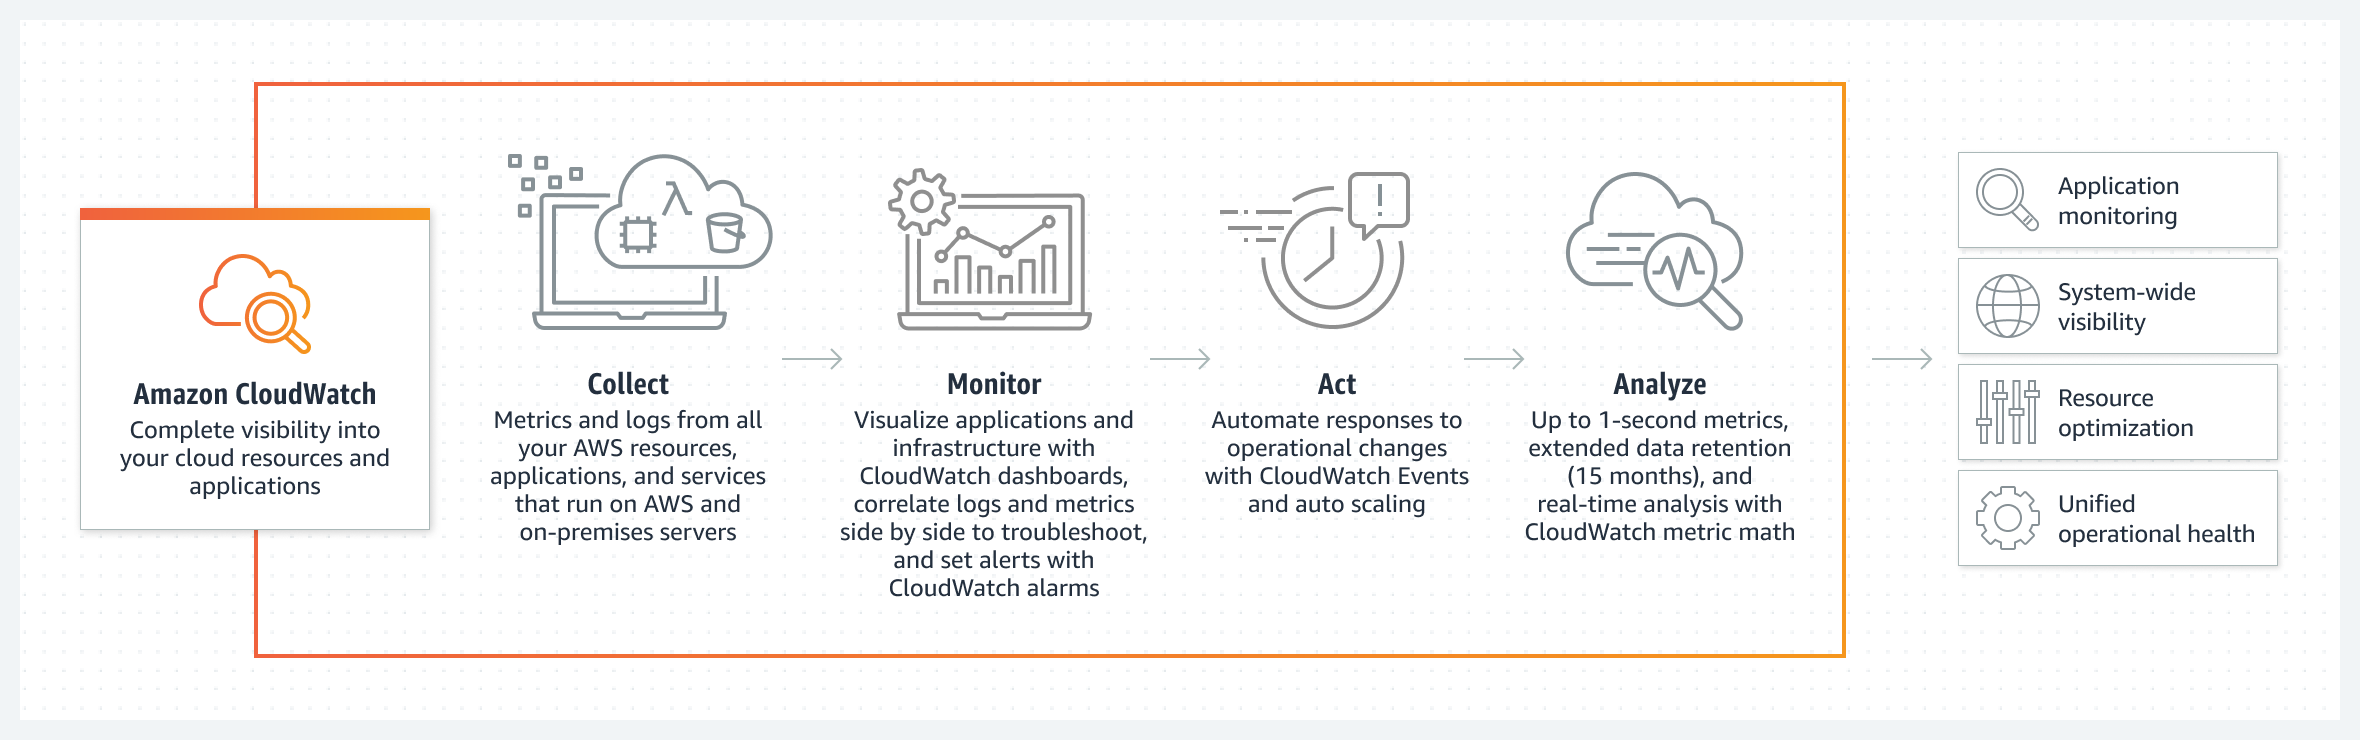
\includegraphics[width=\textwidth,height=6cm,keepaspectratio=true]{images/cloudwatch.png}
            \caption\small{Image Retrieved from: https://aws.amazon.com/cloudwatch/}
            \label{fig:cw}
        \end{figure}
            



	\pagebreak


\section{How to run the code} \label{sec:runcode}
	\paragraph{} To run the main.py correctly, you should already have a keyPairName and securityGroup created in your AWS. After that 
	change the variables to the corresponding value that you have in your AWS. Don't forget to also change the value
	of awsAccessKeyId, secretAccessKey and sessionToken too! Right after this, all you have to do is run the main.py. It will then
	create everything you need and install/setup Flask into each instance, alongside the load balancer and clusters. 
	\bigskip


\section{References} \label{sec:references}
	
	\begin{thebibliography} {}
		\bibitem{1} S. A. Abtahizadeh, \emph{LOG8415: Lab 1 Selecting VM instances in the Cloud through benchmarking}, LOG8415: Advanced Concepts of Cloud Computing, 2019.
		\bibitem{2} Amazon Web Services. (2019) Amazon EC2. \url{https://aws.amazon.com/ec2/}
		\bibitem{3} Amazon Web Services. (2019) Amazon EC2 Instance Types. \url{https://aws.amazon.com/ec2/instance-types/}
		\bibitem{4} Dyouri,A. (2020). How To Make a Web Application Using Flask in Python 3. Digital Ocean.  \url{https://www.digitalocean.com/community/tutorials/how-to-make-a-web-application-using-flask-in-python-3}
		\bibitem{5} Amazon. (n.d). CloudWatch metrics for your Application Load Balancer. AWS. \url{https://docs.aws.amazon.com/elasticloadbalancing/latest/application/load-balancer-cloudwatch-metrics.html}
		\bibitem{6} Amazon. (n.d). CloudWatch. AWS boto3. \url{https://boto3.amazonaws.com/v1/documentation/api/latest/reference/services/cloudwatch.html}
	\end{thebibliography}

\end{document}
